\documentclass[11pt,a4paper]{article}

% --- Essential Packages ---
\usepackage[utf8]{inputenc}
\usepackage[T1]{fontenc}
\usepackage{lmodern}
\usepackage[margin=1in]{geometry}
\usepackage{setspace}
\setstretch{1.18}

\usepackage{amsmath,amssymb,amsfonts}
\usepackage{graphicx}
\usepackage{booktabs}
\usepackage{tabularx}
\usepackage{multirow}
\usepackage{caption}
\usepackage{subcaption}
\usepackage{fancyhdr}
\usepackage{microtype}
\usepackage{xcolor}
\usepackage{cite}
\usepackage{enumitem}

% Float handling parameters to prevent dense clumps or orphaned float pages
\renewcommand{\topfraction}{0.90}
\renewcommand{\bottomfraction}{0.85}
\renewcommand{\textfraction}{0.10}
\renewcommand{\floatpagefraction}{0.80}
\setlength{\floatsep}{12pt plus 2pt minus 2pt}
\setlength{\textfloatsep}{14pt plus 2pt minus 4pt}
\setlength{\intextsep}{12pt plus 2pt minus 2pt}

% Hyperref setup with elegant academic colors
\usepackage[
    colorlinks=true,
    linkcolor=blue!70!black,
    citecolor=green!50!black,
    urlcolor=blue!80!black,
    pdfauthor={Md. Jubayer Hossain},
    pdftitle={metaXpress: reproducible, validated meta-analysis of bulk RNA-seq studies}
]{hyperref}

% Header and Footer styling
\pagestyle{fancy}
\fancyhf{}
\fancyhead[L]{\small\textit{metaXpress: Multi-Cohort Bulk RNA-seq Meta-Analysis}}
\fancyhead[R]{\small\textit{Preprint}}
\fancyfoot[C]{\thepage}
\renewcommand{\headrulewidth}{0.4pt}
\renewcommand{\footrulewidth}{0pt}

% Caption styling
\captionsetup{
    font=small,
    labelfont=bf,
    format=plain,
    justification=justified,
    singlelinecheck=false,
    skip=8pt
}

% Section title aesthetics
\usepackage{titlesec}
\titleformat{\section}{\large\bfseries\color{blue!80!black}}{\thesection}{1em}{}[\titlerule]
\titleformat{\subsection}{\normalsize\bfseries\color{black}}{\thesubsection}{1em}{}
\titleformat{\subsubsection}{\small\bfseries\color{black!80}}{\thesubsubsection}{1em}{}
\titlespacing*{\section}{0pt}{10pt plus 2pt minus 2pt}{5pt plus 1pt minus 1pt}
\titlespacing*{\subsection}{0pt}{8pt plus 2pt minus 2pt}{4pt plus 1pt minus 1pt}
\titlespacing*{\subsubsection}{0pt}{6pt plus 1pt minus 1pt}{3pt plus 1pt minus 1pt}

% ------------------------------------------------------------------------------
% Document Information
% ------------------------------------------------------------------------------
\title{\vspace{-1.5cm}\Large\textbf{metaXpress: reproducible and validated meta-analysis of bulk RNA-seq studies in R}\vspace{0.4cm}}

\author{
    \textbf{Md. Jubayer Hossain}$^{1, 2, *}$\\[0.3cm]
    $^{1}$Center for Health Innovation, Research, Action, and Learning - Bangladesh\\
    $^{2}$DeepBio\\[0.2cm]
    $^{*}$\small Corresponding author: \texttt{hossainmj.me@gmail.com}
}

\date{}

% ------------------------------------------------------------------------------
% Main Document
% ------------------------------------------------------------------------------
\begin{document}

\maketitle

\begin{abstract}
\noindent\textbf{Background:} Meta-analysis of independent bulk RNA-seq studies increases power and separates reproducible signals from study-specific effects. In practice it requires many separate steps: data retrieval, quality control, identifier harmonisation, per-study differential expression (DE), statistical pooling, heterogeneity and robustness assessment, and pathway interpretation. Each hand-off between tools is a source of error.\\
\textbf{Methods:} \texttt{metaXpress} is an R package that implements this workflow on Bioconductor data structures. It retrieves uniformly processed raw counts from the NCBI GEO RNA-seq pipeline. It records data-level quality criteria as pass, fail or not evaluable, and runs per-study DE with DESeq2, edgeR or limma-voom using covariates and explicit contrasts. Results are combined with nine gene-level methods:
\begin{itemize}[noitemsep,topsep=1pt]
    \item random effects with REML, Paule--Mandel or DerSimonian--Laird $\tau^2$, optionally with the Hartung--Knapp--Sidik--Jonkman (HKSJ) adjustment, reporting confidence and prediction intervals;
    \item a fixed (common) effect model;
    \item directional Fisher, Stouffer and weighted inverse-normal combination;
    \item minP, maxP and the $r$-th ordered p-value (rOP);
    \item AWmeta.
\end{itemize}
The package also provides leave-one-out robustness analysis, small-study tests, gene-set enrichment of the meta-signature, cross-study pathway meta-analysis and downstream analyses (transcription-factor activity, cell composition, consensus co-expression, drug-signature reversal).\\
\textbf{Results:} On 300 genes from real data, random-effects estimates, standard errors, $\tau^2$ and p-values agreed with \texttt{metafor} to within $1.6\times10^{-10}$, and per-study DE reproduced native DESeq2 exactly.
\begin{itemize}[noitemsep,topsep=1pt]
    \item \emph{Alzheimer's disease (AD).} Four independent post-mortem brain cohorts (340 brains; two donor-overlapping series excluded) gave 7,491 genes at FDR $\le 0.05$. These recover established glial up-regulation (GFAP, C4B) and neuronal/neuropeptide loss (VIP, VGF, BDNF, CRH, NPTX2). For 2,133 genes the 95\% prediction interval excludes zero, and 1,239 remain significant after removing any single cohort. Pathways show loss of oxidative phosphorylation and gain of inflammatory signalling.
    \item \emph{Pancreatic ductal adenocarcinoma (PDAC).} Three cohorts implicate NF-$\kappa$B/AP-1 activity, myeloid and fibroblast enrichment, and an MST1R-centred epithelial module. Among 5,425 compounds, TGF-$\beta$ receptor inhibitors and erlotinib are top reversers of the tumour signature.
\end{itemize}
The case studies also show practical limits. With four studies, HKSJ-adjusted tests cannot reach genome-wide significance, and a single large cohort dominates many findings.\\
\textbf{Availability:} MIT-licensed at \url{https://github.com/hossainlab/metaXpress}, with executable vignettes on the data analysed here.
\end{abstract}

\vspace{0.2cm}
\noindent\textbf{Keywords:} Bulk RNA-seq, meta-analysis, differential expression, random-effects model, heterogeneity, prediction interval, Bioconductor.

\vspace{0.4cm}

% ==============================================================================
\section{Introduction}
% ==============================================================================
Individual bulk RNA-seq studies are often small, and genome-wide multiple-testing correction then leaves many true effects undetected. Results also depend on cohort, tissue sampling and laboratory protocol. Combining independent studies can increase power and, more importantly, can distinguish effects that replicate from those that do not \cite{rau2014metarnaseq}.

Several R packages address parts of this task:
\begin{itemize}[noitemsep,topsep=2pt]
    \item \texttt{MetaDE} provides quality control and DE meta-analysis for microarray data \cite{wang2012metade}.
    \item \texttt{metaRNASeq} combines per-study p-values from RNA-seq \cite{rau2014metarnaseq}.
    \item \texttt{DExMA} addresses genes missing from some studies \cite{villatorogarcia2022dexma}.
    \item \texttt{metafor} implements general effect-size meta-analysis \cite{viechtbauer2010metafor}.
    \item \texttt{AWFisher} provides adaptive weighting \cite{huo2020awfisher}.
\end{itemize}
A complete analysis still requires the user to assemble data retrieval, quality control, identifier mapping, per-study DE, the choice of pooling model, heterogeneity and robustness checks, and pathway interpretation. Each step has known pitfalls:
\begin{itemize}[noitemsep,topsep=2pt]
    \item fold changes with inconsistent contrast orientation;
    \item standard errors on mixed logarithmic scales;
    \item donors shared between studies;
    \item batch-corrected values fed into count models;
    \item p-value combinations that accumulate evidence from opposite directions;
    \item significance reported without regard to between-study heterogeneity.
\end{itemize}

\texttt{metaXpress} implements the whole workflow on Bioconductor \texttt{SummarizedExperiment} objects \cite{huber2015orchestrating, morgan_se}. It makes these decisions explicit and tests its statistical core against reference implementations. Here we describe its design and validation, and apply it to two public datasets: AD brain tissue and PDAC.

% ==============================================================================
\section{Design and implementation}
% ==============================================================================

\begin{figure}[!htbp]
    \centering
    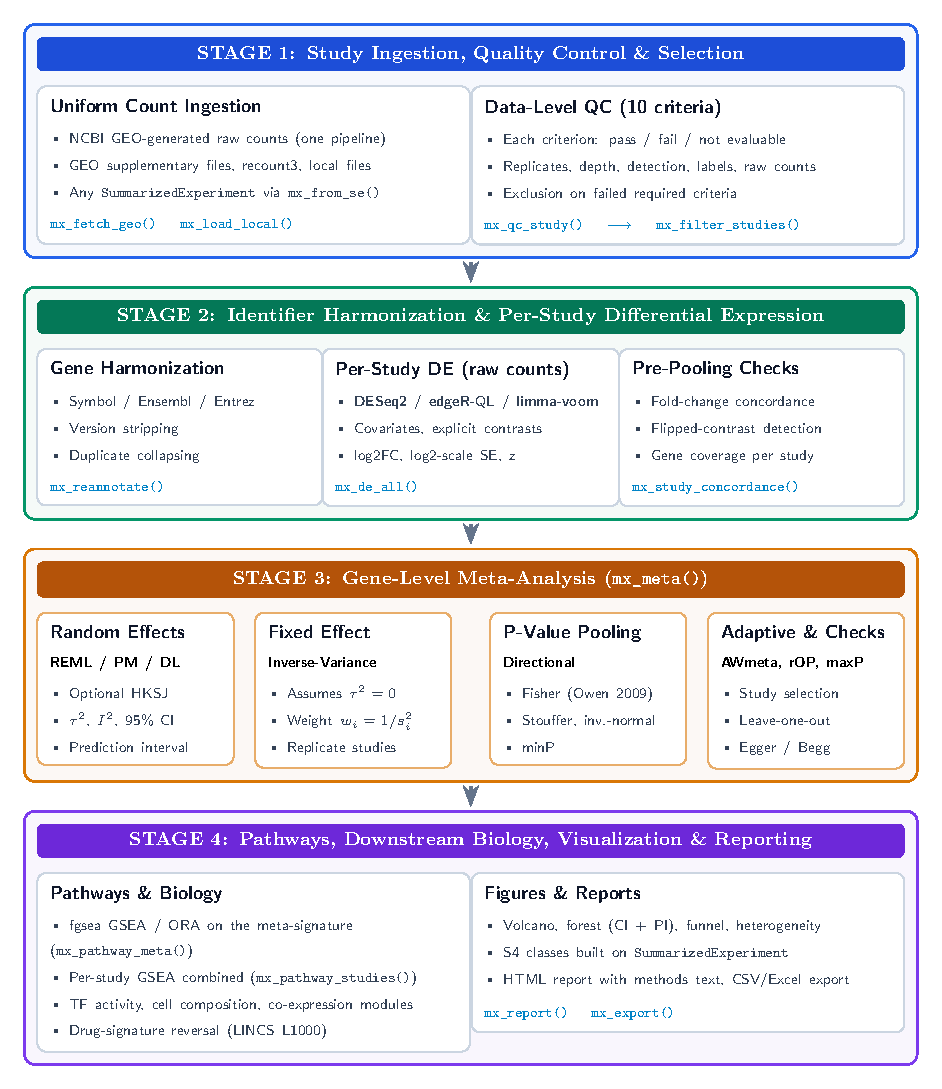
\includegraphics[width=0.86\linewidth]{figures/fig1_architecture.pdf}
    \caption{\textbf{Architecture of \texttt{metaXpress}.} Studies enter as \texttt{metaXpressStudy} objects (a \texttt{SummarizedExperiment} subclass) holding raw counts and sample annotation. They are quality-controlled and harmonised, and differential expression is computed separately in each study from raw counts. The per-study results are pooled into a \texttt{metaXpressResult}, which feeds robustness checks, pathway and downstream analyses, figures and reports.}
    \label{fig:workflow}
\end{figure}

\subsection{Data ingestion and quality control}
\texttt{mx\_fetch\_geo()} retrieves raw counts generated by the NCBI GEO RNA-seq pipeline \cite{clough2024geo}. This pipeline re-processes the SRA reads of eligible human and mouse series with a single alignment (HISAT2 to GRCh38.p13 or GRCm39) and gene counting (featureCounts on RefSeq) protocol. Using these counts removes differences in aligner, annotation and count definition between studies. Series without NCBI counts fall back to author-supplied files. Count matrices from local files, \texttt{recount3} or any \texttt{SummarizedExperiment} are also accepted. The case/control phenotype column is specified explicitly; automatic detection is only a fallback.

\texttt{mx\_qc\_study()} records ten data-level criteria as \emph{pass}, \emph{fail} or \emph{not evaluable}:
\begin{itemize}[noitemsep,topsep=2pt]
    \item at least three samples per group \cite{schurch2016replicates};
    \item median assigned reads;
    \item alignment, rRNA and duplicate rates (if supplied);
    \item gene detection;
    \item complete condition labels;
    \item a two-group contrast;
    \item batch--condition aliasing \cite{leek2010batch};
    \item untransformed integer counts.
\end{itemize}
The score is the number of criteria passed and is never rescaled over the evaluable criteria, so missing information cannot inflate it. \texttt{mx\_filter\_studies()} excludes studies that fail criteria required for valid count-based DE: replicates, labels and raw counts. These checks complement, and do not replace, an assessment of study-level reporting quality \cite{heberle2024ad}.

\subsection{Identifier harmonisation and pre-pooling checks}
\texttt{mx\_reannotate()} maps gene symbols, Ensembl and Entrez identifiers using organism annotation packages (human, mouse, rat) or a user-supplied table. It removes Ensembl version suffixes and detects the identifier type from all IDs. When several source IDs map to one gene, it keeps the most highly expressed row (or sums or drops them), so gene names are unique \cite{miller2011collapserows}.

Before pooling, \texttt{mx\_study\_concordance()} computes pairwise fold-change correlations between studies. A negative correlation almost always indicates a reversed case/control contrast. Genes not measured in a study are treated as missing, not as zero effects, and each gene is pooled over the studies that measured it. Imputation from other studies is discouraged because it inflates the apparent number of studies and deflates heterogeneity.

\subsection{Per-study differential expression}
\texttt{mx\_de()} fits DESeq2 \cite{love2014deseq2}, edgeR quasi-likelihood \cite{robinson2010edger, chen2016edgerql} or limma-voom \cite{law2014voom, ritchie2015limma} models to raw counts. The design formula may include covariates, and an explicit contrast fixes the orientation of every fold change (case/control).

All engines return a common table: log$_2$ fold change $y_i$, its standard error $s_i$ on the log$_2$ scale, a signed z-statistic, p-values and group sizes.
\begin{itemize}[noitemsep,topsep=2pt]
    \item \emph{DESeq2:} the unshrunken maximum-likelihood estimate and its standard error are retained, because inverse-variance pooling requires them. Shrunken estimates \cite{zhu2019apeglm} are stored separately for ranking.
    \item \emph{edgeR:} the GLM coefficients are on the natural-log scale, so $s_i$ is obtained from the quasi-likelihood test as $|y_i|/|z_i|$ with $z_i = \Phi^{-1}(1-p_i/2)$.
    \item \emph{limma:} $s_i$ is the moderated standard error.
\end{itemize}
Normalisation and between-study batch correction (ComBat-seq, ComBat, \texttt{removeBatchEffect}, with the condition effect preserved) write new assays and never overwrite raw counts \cite{zhang2020combatseq}. Because DE is computed within studies, between-study batch effects do not enter the per-study estimates. Batch correction is therefore reserved for pooled visualisation \cite{nygaard2016batch}.

\subsection{Gene-level meta-analysis}
\texttt{mx\_meta()} implements two families of methods, which answer different questions (Table~\ref{tab:methods}).

\paragraph{Effect-size models.} The fixed (common) effect estimate is $\hat\theta_{\mathrm{FE}} = \sum w_i y_i/\sum w_i$ with $w_i = 1/s_i^2$. The random-effects model assumes $y_i \sim N(\theta, s_i^2 + \tau^2)$:
\begin{equation}
    \hat\theta_{\mathrm{RE}} = \frac{\sum_i w_i^* y_i}{\sum_i w_i^*}, \qquad w_i^* = \frac{1}{s_i^2 + \hat\tau^2}, \qquad \mathrm{SE}(\hat\theta_{\mathrm{RE}}) = \Big(\sum_i w_i^*\Big)^{-1/2}.
\end{equation}
The between-study variance $\tau^2$ is estimated per gene by one of three methods \cite{veroniki2016methods, langan2019comparison}:
\begin{itemize}[noitemsep,topsep=2pt]
    \item restricted maximum likelihood (REML; Fisher scoring) \cite{viechtbauer2005bias}, the default;
    \item Paule--Mandel, solving $\sum_i w_i^*(y_i-\hat\theta)^2 = k-1$ \cite{paule1982consensus};
    \item DerSimonian--Laird \cite{dersimonian1986meta}.
\end{itemize}
The HKSJ adjustment replaces the standard error by
\[
\big[\sum_i w_i^*(y_i-\hat\theta)^2/\{(k-1)\sum_i w_i^*\}\big]^{1/2}
\]
and uses a $t_{k-1}$ reference \cite{hartung2001refined, inthout2014hksj}. Each gene receives Cochran's $Q$, $I^2 = \max\{0, (Q-k+1)/Q\}$ \cite{higgins2002quantifying}, $\hat\tau^2$, a 95\% confidence interval and a 95\% prediction interval
\[
\hat\theta \pm t_{k-2}\sqrt{\hat\tau^2 + \mathrm{SE}^2},
\]
which is the expected range of the effect in a new study \cite{higgins2009reevaluation}.

\paragraph{Combination of evidence.} Two-sided p-values are converted to one-sided values using the sign of $y_i$. The combination methods are:
\begin{itemize}[noitemsep,topsep=2pt]
    \item \emph{Directional Fisher} combines the two one-sided Fisher tests (Pearson's test; \cite{owen2009pearson}), so evidence in opposite directions does not accumulate.
    \item \emph{Stouffer and weighted inverse-normal} combine signed z-scores, the latter with $\sqrt{n_i}$ weights \cite{marot2009moderated, rau2014metarnaseq}.
    \item \emph{minP, maxP and rOP} test whether a gene is DE in at least one, all, or at least $r$ studies, using $p_{(r)} \sim \mathrm{Beta}(r, k-r+1)$ \cite{song2014rop}.
    \item \emph{AWmeta} \cite{hu2026awmeta} selects, for each gene, the subset of studies that minimises the Fisher statistic. The resulting AW-Fisher p-value \cite{li2011awfisher} is calibrated with \texttt{AWFisher} \cite{huo2020awfisher}, and the effect is estimated by REML random effects over the selected studies. The selected studies are reported for each gene.
\end{itemize}
For all methods, p-values are adjusted across genes by the Benjamini--Hochberg procedure.

\begin{table}[!htbp]
\centering
\small
\caption{\textbf{Gene-level meta-analysis methods in \texttt{mx\_meta()}.} Methods answer different questions and should be chosen a priori.}
\label{tab:methods}
\begin{tabularx}{\textwidth}{l l >{\raggedright\arraybackslash}X}
\toprule
\textbf{Method} & \textbf{\texttt{method =}} & \textbf{Hypothesis / estimand} \\
\midrule
Random effects (REML / PM / DL, optional HKSJ) & \texttt{random\_effects} & Average log$_2$FC across populations, with $\tau^2$, $I^2$, CI and prediction interval \\
Fixed (common) effect & \texttt{fixed\_effects} & A single shared log$_2$FC (studies are replicates) \\
Directional Fisher & \texttt{fisher} & Same-direction effect in at least one study \\
Stouffer & \texttt{stouffer} & Signed evidence, equal weights \\
Weighted inverse-normal & \texttt{inverse\_normal} & Signed evidence, $\sqrt{n}$ weights \\
minP / maxP / rOP & \texttt{minp}, \texttt{maxp}, \texttt{rop} & DE in $\ge 1$, all, or $\ge r$ studies \\
AWmeta & \texttt{awmeta} & DE in an adaptively selected subset of studies \\
\bottomrule
\end{tabularx}
\end{table}

\subsection{Robustness, small-study effects and visualisation}
\texttt{mx\_sensitivity()} repeats the analysis leaving out each study in turn. For every gene it reports the fraction of runs that remain significant with the same direction.

\texttt{mx\_small\_study()} runs per-gene Egger regression \cite{egger1997bias} and Begg--Mazumdar rank-correlation tests \cite{begg1994operating}. It warns that both tests have little power with fewer than ten studies \cite{sterne2011recommendations}.

Forest plots show the pooled confidence interval and prediction interval. Funnel, volcano, heterogeneity and UpSet plots, an HTML report with generated methods text, and tabular export are provided.

\subsection{Pathway and downstream analyses}
\texttt{mx\_pathway\_meta()} runs pre-ranked GSEA (\texttt{fgsea} \cite{korotkevich2016fgsea, subramanian2005gsea}) on the signed meta-analysis z-score with MSigDB collections \cite{liberzon2015hallmark}. It can instead run over-representation analysis separately for up- and down-regulated genes against the tested universe.

\texttt{mx\_pathway\_studies()} runs GSEA in each study and combines the pathway p-values with a directional Stouffer test, in the spirit of MAPE \cite{shen2010mape}.

Module 9 provides four downstream analyses:
\begin{itemize}[noitemsep,topsep=2pt]
    \item transcription-factor activity from the meta z-score with CollecTRI regulons and a univariate linear model \cite{muellerdott2023collectri, badiaimompel2022decoupler};
    \item cell-type composition shifts from MCP-counter markers \cite{becht2016mcpcounter}, pooled as Hedges' $g$ across studies;
    \item consensus co-expression modules, whose co-expression must hold in every study \cite{langfelder2008wgcna};
    \item drug-signature reversal against LINCS L1000 consensus signatures \cite{subramanian2017l1000, lamb2006cmap}.
\end{itemize}

\subsection{Software validation}
The test suite checks the statistical core against reference implementations:
\begin{itemize}[noitemsep,topsep=2pt]
    \item random- and fixed-effect results (all $\tau^2$ estimators, with and without HKSJ) against \texttt{metafor::rma()} \cite{viechtbauer2010metafor};
    \item Egger and Begg tests against \texttt{metafor::regtest()} and \texttt{ranktest()};
    \item AWmeta against \texttt{AWFisher} combined with \texttt{metafor};
    \item p-value combinations against their closed forms;
    \item per-study DE against native DESeq2 on the airway dataset (GEO GSE52778; \cite{himes2014airway}).
\end{itemize}
All numbers and figures in this article are produced by \nolinkurl{scripts/make_preprint_results.R}.

% ==============================================================================
\section{Results}
% ==============================================================================

\subsection{Agreement with reference implementations}
For 300 randomly chosen genes from the AD data, \texttt{metaXpress} and \texttt{metafor} were compared across all six random-effects configurations (DL, REML, PM, each with and without HKSJ). Pooled effects, standard errors, $\tau^2$ and p-values differed by at most $1.6\times10^{-10}$.

This comparison exposed one design decision that matters in practice. DESeq2 reports a fold change but no p-value for count outliers flagged by Cook's distance. \texttt{metaXpress} treats such genes as not measured in that study (191 genes in GSE53697), and identical results are obtained only when the reference analysis does the same.

On airway, \texttt{mx\_de()} with a paired design (donor cell line as a covariate) reproduced native DESeq2 fold changes exactly. Fold changes from DESeq2, edgeR and limma-voom correlated at $r \ge 0.997$.

\subsection{Case study 1: Alzheimer's disease brain tissue}

\paragraph{Study selection and independence.} We selected GEO series of human post-mortem brain bulk RNA-seq comparing AD with non-demented controls, for which NCBI-processed counts were available (Table~\ref{tab:ad}).

Two candidate series were excluded because they share donors with included series:
\begin{itemize}[noitemsep,topsep=2pt]
    \item GSE95587 (fusiform gyrus): 89 of its 117 case identifiers also occur in GSE125583;
    \item GSE159699: built from the same brain-bank donors as GSE104704.
\end{itemize}
Pooling these would count the same individuals twice.

Per-study models were DESeq2 with sex as a covariate where available. Genes were restricted to protein-coding genes with $\ge 10$ counts in at least as many samples as the smaller group. The control group of GSE104704 was restricted to aged controls. NCBI processed only 12 of the 17 libraries deposited for GSE53697.

\begin{table}[!htbp]
\centering
\small
\caption{\textbf{Alzheimer's disease cohorts.} DEGs: per-study genes at FDR $\le 0.05$ (DESeq2).}
\label{tab:ad}
\begin{tabular}{l l r r r r}
\toprule
\textbf{GEO} & \textbf{Region} & \textbf{AD} & \textbf{Control} & \textbf{Genes} & \textbf{DEGs} \\
\midrule
GSE125583 \cite{srinivasan2020gse125583} & Fusiform gyrus & 218 & 70 & 16,126 & 10,164 \\
GSE104704 \cite{nativio2018gse104704} & Lateral temporal lobe & 12 & 10 & 15,930 & 1,670 \\
GSE53697 \cite{scheckel2016gse53697} & Dorsolateral prefrontal cortex & 6 & 6 & 16,029 & 1 \\
GSE173955 \cite{gse173955ref} & Hippocampus & 8 & 10 & 15,905 & 4,149 \\
\bottomrule
\end{tabular}
\end{table}

\paragraph{Concordance.} Fold changes of the three larger cohorts were strongly correlated (Spearman $r = 0.68$--$0.80$ over genes significant in either study). The small prefrontal cohort correlated weakly but positively ($0.09$--$0.39$), so no contrast was reversed.

\paragraph{Meta-analysis.} A random-effects model with REML $\tau^2$ was chosen a priori, to estimate the average effect across regions and cohorts that are expected to differ.

Of 16,290 genes tested (15,107 measured in all four studies), 7,491 had meta FDR $\le 0.05$ (3,585 up, 3,906 down; Figure~\ref{fig:ad}A), with a median $I^2$ of 15\%. For 2,133 of these genes the 95\% prediction interval excluded zero, so the same direction of change is expected in a new cohort.

The analysis recovered established AD biology (Table~\ref{tab:genes}, Figure~\ref{fig:ad}B):
\begin{itemize}[noitemsep,topsep=2pt]
    \item \emph{Up:} the astrocyte marker GFAP was homogeneously up-regulated ($I^2 = 0$, prediction interval excluding zero), as were the complement gene C4B and CD44.
    \item \emph{Down:} neuronal and neuropeptide genes VIP, VGF, BDNF, CRH and NPTX2 were down-regulated.
\end{itemize}
Many of these genes were strongly heterogeneous. The interneuron markers SST and PVALB showed large losses in some cohorts but $I^2 \ge 87\%$ and were not significant on average. This pattern is consistent with region-dependent neuronal loss in the sampled tissue, and it illustrates why significance should be reported together with heterogeneity.

\begin{figure}[!htbp]
    \centering
    \begin{subfigure}[b]{0.47\linewidth}
        \centering
        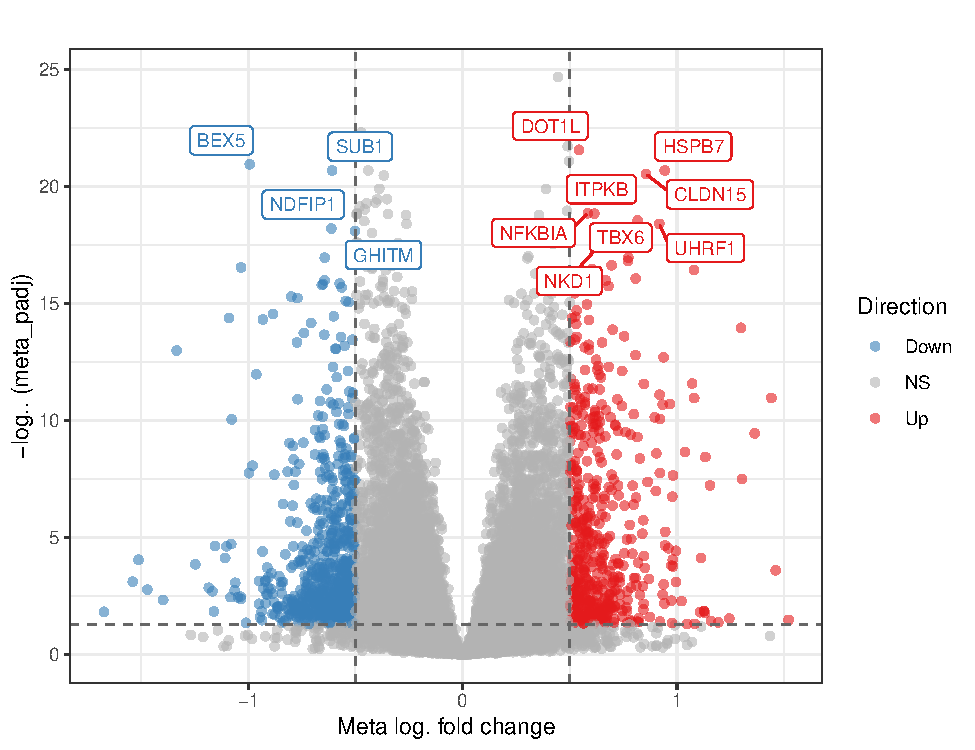
\includegraphics[width=\linewidth]{figures/fig2_ad_volcano.pdf}
        \caption{}
    \end{subfigure}
    \hfill
    \begin{subfigure}[b]{0.50\linewidth}
        \centering
        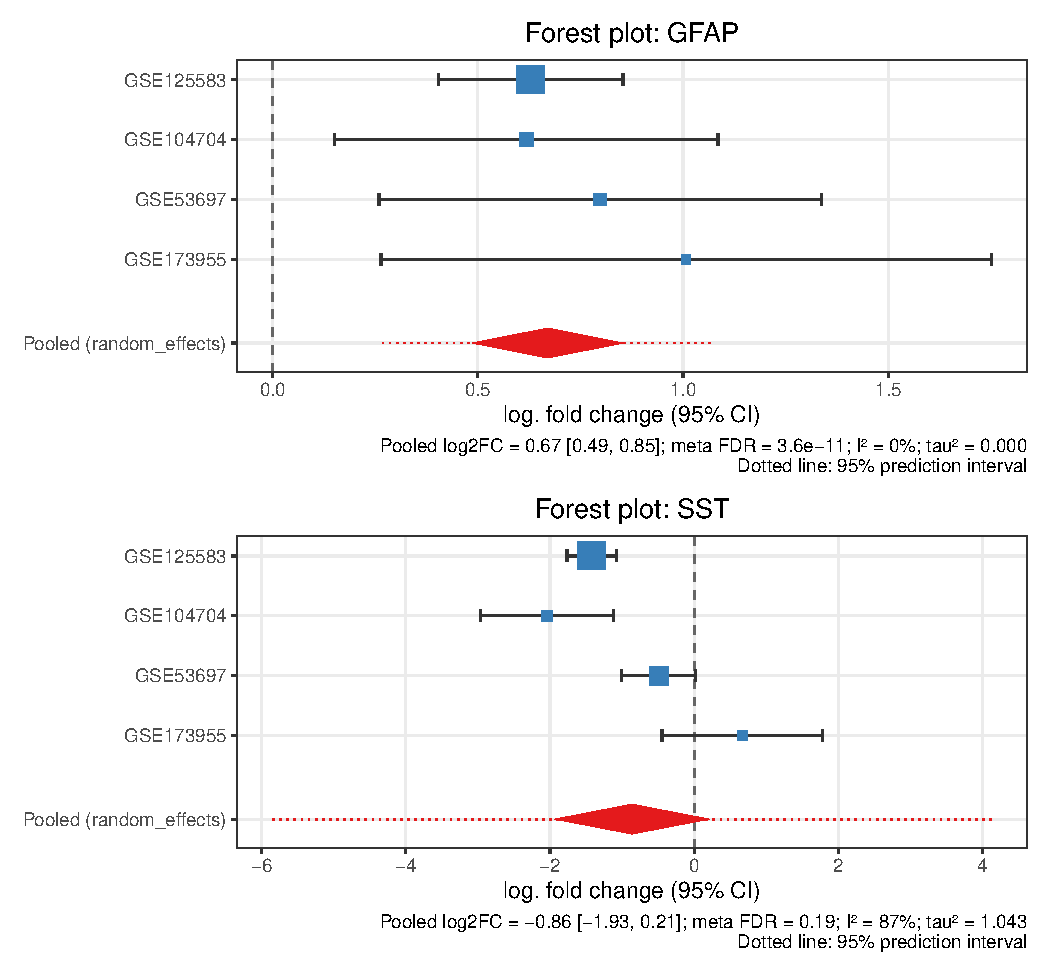
\includegraphics[width=\linewidth]{figures/fig3_ad_forest.pdf}
        \caption{}
    \end{subfigure}
    \caption{\textbf{Alzheimer's disease meta-analysis (random effects, REML).} (A) Meta-analysis volcano plot. Dashed lines: meta FDR $= 0.05$ and $|\log_2\mathrm{FC}| = 0.5$. (B) Forest plots for GFAP (homogeneous; the prediction interval, dotted, excludes zero) and SST (heterogeneous, $I^2 = 87\%$; not significant on average). Squares are proportional to inverse-variance weight; diamonds show the pooled 95\% confidence interval.}
    \label{fig:ad}
\end{figure}

\begin{table}[!htbp]
\centering
\footnotesize
\caption{\textbf{Selected established AD genes.} Pooled log$_2$FC (AD/control) with 95\% confidence interval (CI) and 95\% prediction interval (PI), random effects with REML $\tau^2$.}
\label{tab:genes}
\begin{tabular}{l r c c r r}
\toprule
\textbf{Gene} & \textbf{log$_2$FC} & \textbf{95\% CI} & \textbf{95\% PI} & \textbf{FDR} & \textbf{$I^2$ (\%)} \\
\midrule
GFAP  & $0.67$  & $[0.49, 0.85]$   & $[0.27, 1.07]$   & $3.6\times10^{-11}$ & 0 \\
C4B   & $0.44$  & $[0.23, 0.64]$   & $[-0.01, 0.88]$  & $1.4\times10^{-4}$ & 31 \\
CD44  & $0.48$  & $[0.12, 0.85]$   & $[-0.54, 1.51]$  & $0.023$ & 38 \\
VIP   & $-0.61$ & $[-0.81, -0.41]$ & $[-1.04, -0.18]$ & $2.8\times10^{-8}$ & 0 \\
VGF   & $-1.47$ & $[-2.29, -0.66]$ & $[-5.19, 2.25]$  & $0.0017$ & 86 \\
BDNF  & $-0.85$ & $[-1.30, -0.39]$ & $[-2.80, 1.11]$  & $0.0011$ & 73 \\
CRH   & $-1.54$ & $[-2.34, -0.74]$ & $[-5.05, 1.97]$  & $7.6\times10^{-4}$ & 76 \\
NPTX2 & $-1.04$ & $[-1.65, -0.42]$ & $[-3.75, 1.68]$  & $0.0033$ & 79 \\
SST   & $-0.86$ & $[-1.93, 0.21]$  & $[-5.85, 4.12]$  & $0.19$ & 87 \\
PVALB & $-0.78$ & $[-1.97, 0.40]$  & $[-6.31, 4.74]$  & $0.29$ & 88 \\
\bottomrule
\end{tabular}
\end{table}

\paragraph{Choice of method matters.} Methods that ignore between-study variance call many more genes (Table~\ref{tab:compare}). With one cohort of 288 brains, these calls largely reflect that cohort.

AWmeta makes this explicit. Of its significant genes, 2,424 were supported by GSE125583 alone and only 381 by all four studies. AWmeta also called SST significant, because it selects the two cohorts with a strong loss and ignores the others. This is a different hypothesis from the average effect estimated by random effects.

The HKSJ adjustment is recommended for few studies \cite{inthout2014hksj}, but with $k = 4$ it uses a $t_3$ reference. The smallest observed p-value was $1.3\times10^{-5}$, above the Benjamini--Hochberg threshold for even a single discovery among 16,290 genes ($3.1\times10^{-6}$), so no gene was significant. With few studies, HKSJ is useful for the confidence intervals of prioritised genes but not for genome-wide discovery.

\begin{table}[!htbp]
\centering
\small
\caption{\textbf{Genes at meta FDR $\le 0.05$ in the AD data by method.}}
\label{tab:compare}
\begin{tabular}{l l r}
\toprule
\textbf{Method} & \textbf{Question} & \textbf{Genes} \\
\midrule
Random effects (REML) & Average effect across cohorts & 7,491 \\
Random effects (REML) + HKSJ & Same, small-sample adjusted & 0 \\
Fixed effect & One common effect & 10,861 \\
Weighted inverse-normal & Signed evidence, $\sqrt{n}$ weights & 10,906 \\
Directional Fisher & Same-direction effect in $\ge 1$ study & 10,699 \\
rOP ($r = 2$) & DE in $\ge 2$ of 4 studies & 7,615 \\
maxP & DE in all 4 studies & 1,622 \\
AWmeta & DE in an adaptively selected subset & 10,284 \\
\bottomrule
\end{tabular}
\end{table}

\paragraph{Robustness.} Leaving out GSE125583 reduced the number of significant genes from 7,491 to 1,550. Leaving out any of the other three cohorts left between 5,541 and 8,123 significant genes. A core of 1,239 genes remained significant, with the same direction, after removing any single study. We regard this core as the most defensible AD signature in these data.

Egger tests found no small-study asymmetry among the core genes (0 of 1,239 at FDR $\le 0.05$). With four studies this is not evidence that bias is absent \cite{sterne2011recommendations}.

\paragraph{Pathways.} GSEA of the meta-signature on MSigDB Hallmarks (Figure~\ref{fig:pathways}) showed:
\begin{itemize}[noitemsep,topsep=2pt]
    \item strong loss of oxidative phosphorylation (NES $= -3.08$, FDR $= 4.9\times10^{-31}$) and of MYC targets;
    \item gain of TNF-$\alpha$/NF-$\kappa$B, IL6/JAK/STAT3, p53 and inflammatory-response genes.
\end{itemize}
These match the mitochondrial and neuroinflammatory components of AD pathology. Cross-study pathway meta-analysis gave the same leading themes: oxidative phosphorylation was down-regulated in three of four cohorts. Per-study NES values show that the small prefrontal cohort often diverged from the others.

\begin{figure}[!htbp]
    \centering
    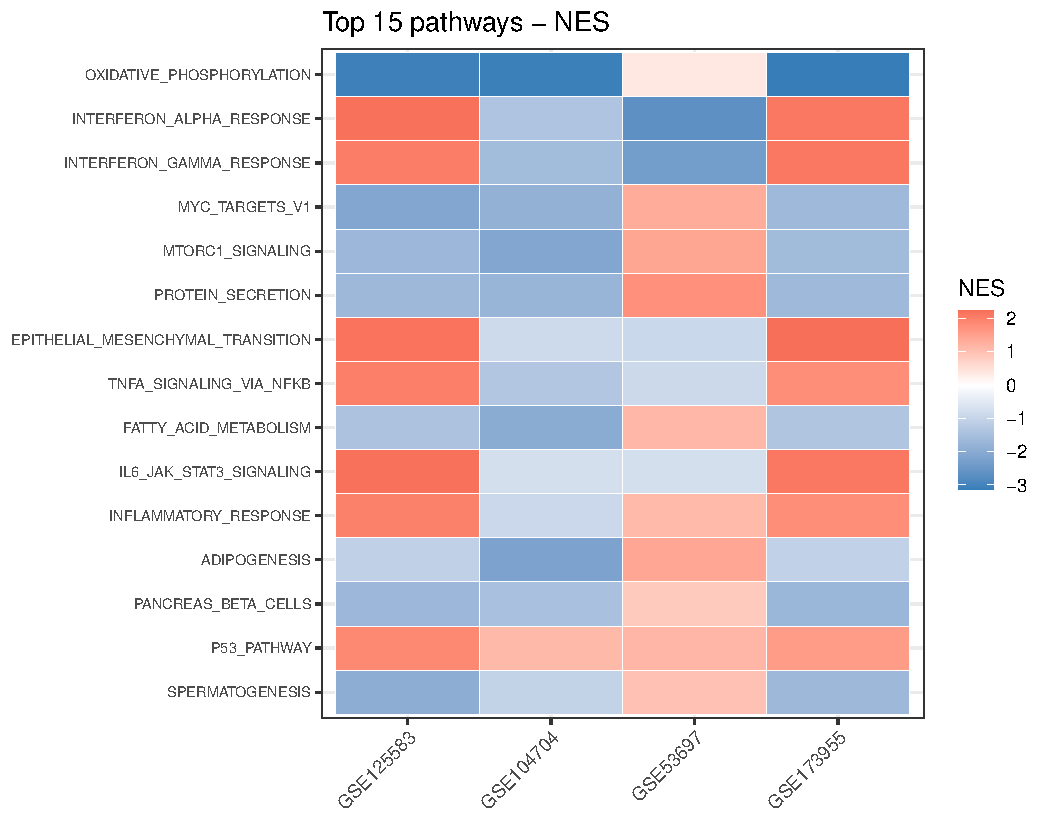
\includegraphics[width=0.66\linewidth]{figures/fig4_ad_pathways.pdf}
    \caption{\textbf{Per-study pathway enrichment in the AD cohorts.} Normalised enrichment scores (fgsea, MSigDB Hallmarks) for the 15 pathways with the largest mean absolute NES. Pathways are combined across studies by directional Stouffer combination in \texttt{mx\_pathway\_studies()}.}
    \label{fig:pathways}
\end{figure}

\subsection{Case study 2: downstream biology in pancreatic ductal adenocarcinoma}
Three GEO cohorts compare PDAC with adjacent non-tumour pancreas:
\begin{itemize}[noitemsep,topsep=2pt]
    \item GSE130688, 15/15 \cite{gse130688ref};
    \item GSE136569, 5/5 \cite{gse136569ref};
    \item GSE171485, 6/6 \cite{gse171485ref}.
\end{itemize}
Tumour/normal labels were taken from the GEO series records. Per-study DESeq2 analyses found 5,863, 146 and 1,105 genes at FDR $\le 0.05$, and fold changes were concordant across cohorts ($r = 0.58$--$0.73$). Random-effects pooling over 29,679 genes identified 1,787 genes with FDR $\le 0.05$ and $|\log_2\mathrm{FC}| \ge 1$ (1,166 up, 621 down).

The downstream analyses (Figure~\ref{fig:pdac}) gave four results.
\begin{itemize}[noitemsep,topsep=2pt]
    \item \emph{Transcription factors.} Of 552 transcription factors scored, 148 were significant. NF-$\kappa$B (RELA, REL, RELB) and AP-1 (JUN) were the most active, followed by E2F, MYC and TP53 targets.
    \item \emph{Cell composition.} Neutrophil, monocytic, myeloid dendritic-cell and fibroblast scores were higher in tumour (pooled Hedges' $g = 0.77$--$1.06$, FDR $\le 0.017$, $I^2 \le 27\%$). This reflects the desmoplastic, myeloid-rich PDAC stroma, and shows that part of the gene-level signature reflects tissue composition.
    \item \emph{Co-expression.} The leading consensus module (398 genes; FDR $= 5.8\times10^{-5}$) was centred on MST1R, PLEK2, TSPAN1, B3GNT3 and CDCP1, a tumour-epithelial programme. A module of acinar genes (CELP, PNLIPRP1, RBPJL) tended to be lost (FDR $= 0.056$).
    \item \emph{Drug reversal.} Among 5,425 LINCS compounds, five of the top eight reversers of the tumour signature inhibit the TGF-$\beta$ type I receptor (SD-208, GW-788388, LY-2109761, LY-364947, SB-525334). The EGFR inhibitor erlotinib, which is approved in combination with gemcitabine for advanced PDAC, ranked fifth.
\end{itemize}
Drug-connectivity p-values assume independent genes and are anti-conservative, so they are used for ranking only.

\begin{figure}[!htbp]
    \centering
    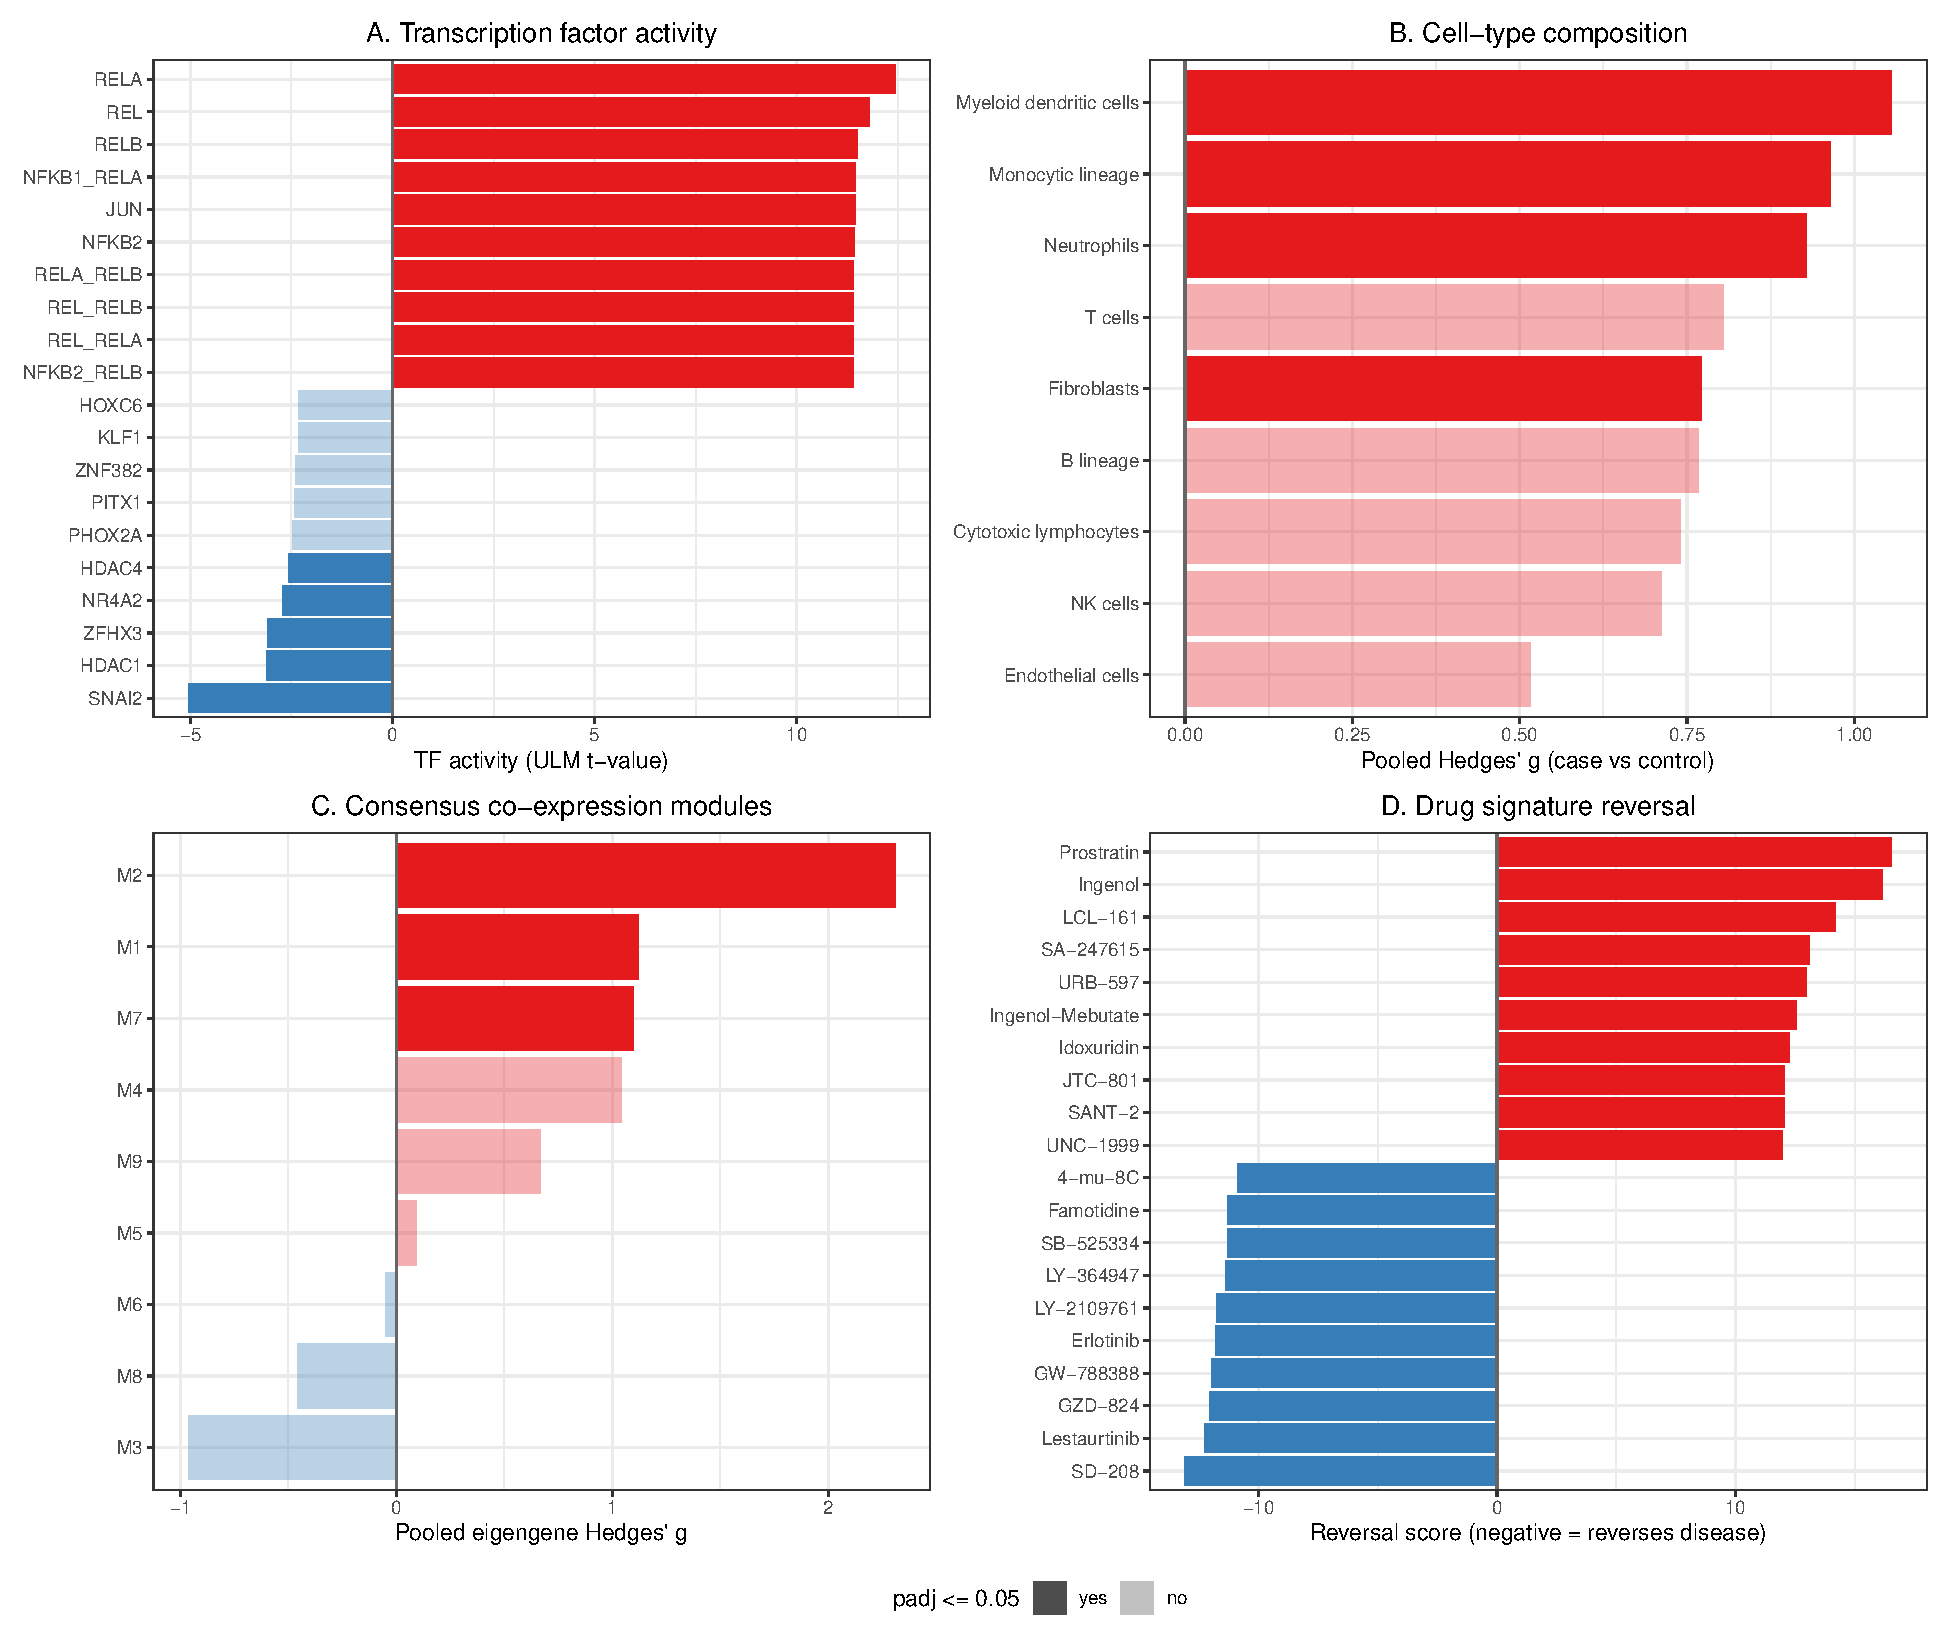
\includegraphics[width=0.95\linewidth]{figures/fig5_pdac_downstream.pdf}
    \caption{\textbf{Downstream biology of the PDAC meta-signature.} (A) Transcription-factor activity (CollecTRI, univariate linear model). (B) Cell-type composition (MCP-counter markers, pooled Hedges' $g$). (C) Consensus co-expression modules (pooled eigengene effect). (D) Drug-signature reversal (LINCS L1000; negative scores reverse the tumour signature). Dark bars: FDR $\le 0.05$.}
    \label{fig:pdac}
\end{figure}

% ==============================================================================
\section{Discussion}
% ==============================================================================
\texttt{metaXpress} brings the steps of a bulk RNA-seq meta-analysis into one workflow and validates its statistical core against reference implementations. The case studies illustrate decisions that strongly affect conclusions but are easy to get wrong:
\begin{itemize}[noitemsep,topsep=2pt]
    \item excluding studies that share donors;
    \item fixing contrast orientation and checking it by concordance;
    \item keeping per-study DE on raw counts;
    \item choosing the pooling model from the scientific question;
    \item reporting heterogeneity, prediction intervals and leave-one-out robustness rather than a single list of significant genes.
\end{itemize}

The AD analysis shows that a meta-analysis with one large cohort is, to a large extent, a re-analysis of that cohort. Most fixed-effect, p-value-based and AWmeta discoveries depended on GSE125583. Prediction intervals and the leave-one-out core distinguish signals that are likely to transfer to new cohorts.

The HKSJ adjustment, despite its good calibration for confidence intervals, cannot support genome-wide discovery when only a handful of studies are available. Researchers should state which question their method answers rather than choose the method that yields the most genes.

\subsection{Limitations}
\begin{itemize}[noitemsep,topsep=2pt]
    \item All methods assume independent studies. Donor overlap must be checked by the analyst; metaXpress cannot detect it automatically.
    \item NCBI uniformly processed counts exist only for eligible human and mouse series. Other data must be harmonised by the user.
    \item Gene-level random-effects inference is approximate when $k$ is small, and the small-study tests are uninformative below about ten studies.
    \item Cell-composition differences can drive tissue-level signatures. Downstream analyses describe associations, and drug-connectivity scores generate hypotheses only.
    \item AWmeta, as originally proposed, does not require the selected studies to agree in direction, so its results should be read together with the reported direction consistency.
\end{itemize}

% ==============================================================================
\section{Code and data availability}
% ==============================================================================
\texttt{metaXpress} is released under the MIT license at \url{https://github.com/hossainlab/metaXpress}. The package includes per-study results for the AD cohorts (\nolinkurl{inst/extdata/ad_brain_de.rds}), built from GEO by \nolinkurl{inst/scripts/make_ad_brain_extdata.R}. Executable vignettes reproduce the analyses.

The PDAC analysis is reproduced by \nolinkurl{scripts/fetch_case_study_data.R} and \nolinkurl{scripts/run_case_study_applications.R}. All values and figures in this article are produced by \nolinkurl{scripts/make_preprint_results.R} (metaXpress 0.99.1, R 4.6.1).

All datasets are public in NCBI GEO under accessions GSE125583, GSE104704, GSE53697, GSE173955, GSE130688, GSE136569, GSE171485 and GSE52778.

% ==============================================================================
\section*{Acknowledgments}
% ==============================================================================
The author thanks members of the Center for Health Innovation, Research, Action, and Learning - Bangladesh and DeepBio for fruitful discussions and software testing.

% ==============================================================================
\section*{Author Contributions}
% ==============================================================================
\textbf{Md. Jubayer Hossain}: Conceptualization, Software, Methodology, Data Curation, Formal Analysis, Validation, Visualization, Writing -- Original Draft, Writing -- Review \& Editing, Project Administration.

% ==============================================================================
\section*{Conflict of Interest}
% ==============================================================================
The author declares no competing financial or non-financial interests.

% ==============================================================================
% References
% ==============================================================================
\begingroup
\footnotesize
\makeatletter
\renewcommand{\@openbib@code}{\setlength{\itemsep}{1pt plus 0.5pt}\setlength{\parsep}{0pt}\setlength{\parskip}{0pt}}
\makeatother
\bibliographystyle{unsrt}
\bibliography{references}
\endgroup

\end{document}
